\begin{frame}{Upside of Policy Gradients}
\begin{columns}
\column {0.55\textwidth}
\begin{itemize}
    \item One of the most attractive thing about policy gradients is that the reward function need not be differentiable with respect to the policy parameters.
    \item This provides us with a framework to handle non differentiable computation when working with neural networks.
    \item Such situation often arises when we require sampling from a probability distribution during the forward pass or when we require to optimize a non differentiable objective function. 
\end{itemize}
\column {0.45\textwidth}
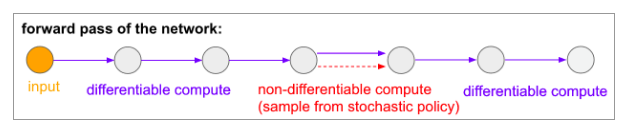
\includegraphics[scale = 0.25]{img/nondiffcomput.png}
\newline
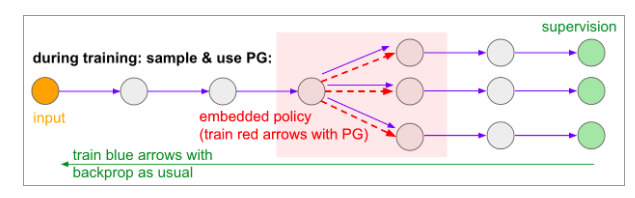
\includegraphics[scale = 0.25]{img/nondiffcomput2.png}
\end{columns}
  \footnotetext[1]{Image from Andrej Karpathy's blog\\ (https://karpathy.github.io/2016/05/31/rl/)}
\end{frame}
\begin{frame}{Case Study: Optimizing BLEU for NMT}
    \begin{itemize}
        \item For training Machine Translation systems we optimize the negative log likelihood of the predictions of decoder.
        \item However NLL loss might not be the best measure of the quality of translation.
        \item For evaluation of the translation by an NMT model we often use metrics like BLEU.
        \item However using standard supervised learning approaches we can not directly optimize BLEU since it requires the access to the predicted tokens, not the probabilities.
        \item To make matters worse BLEU calculation is non differentiable so even if we manage to select the tokens by a differentiable operation (max pool) it will still be problematic.
    \end{itemize}
\end{frame}
\begin{frame}{Case Study: Optimizing BLEU for NMT}
    \begin{itemize}
        \item Policy Gradients to the rescue!
        \item We can represent the machine translation problem as an MDP:
            \begin{itemize}
                \item State $s_t$ : The state at time step $t$ will be given by the input token to the decoder at time $t$ and the hidden state of the decoder $h_t$ which encompasses information from the previous time steps of decoder as well as the hidden states of encoder.
                \item Action $a_t$ : The action at time step $t$ is given by the prediction of decoder at time $t$. This hence becomes a case of discrete action space and we can use a softmax policy.
                \item Reward $r_t$: We use a delayed reward in this case where 0 reward is given at all time steps and at final step reward equal to the BLEU score between the prediction and the ground truth is used.
                \item Transition $\mathbb{P}$ : Transition in this case will be given by the input token at the next time step and the updated hidden state of RNN $h_t$
            \end{itemize}
    \end{itemize}
\end{frame}

\begin{frame}{Case Study: Optimizing BLEU for NMT}
    \begin{itemize}
        \item Now we can simply use the REINFORCE algorithm to train our translation system.
        \item Please note that the action space for this problem is quite large (equal to the number of words in the vocabulary).
        \item Directly training the model with REINFORCE will be very slow and might not even converge to a good policy.
        \item People often first train their model using the standard supervised learning approach and then fine tune it using policy gradients.
    \end{itemize}
\end{frame}